
\section{Discussion}
\label{sec:discussion}
\subsection{The impact of Decay Factor $\lambda$}
\label{sec:discsussion-lambda}
% The decay factor $\lambda$ is an very important hyper-parameter in our scaling law function. We use two kinds of decay factor (0.99 and 0.999) to predict the loss curve of square and 1-sqrt annealing method, and the result is shown in Fig.~\ref{fig:lamda}.  First, the decay factor is larger, the delay steps are longer. The 0.999 decay factor has a longer delay steps than 0.99 delay factor in both annealing methods. 
% Second, the decay factor also decides the relative size of annealing area $S_2$ of square and 1-sqrt annealing area. In the case of 0.999 decay factor, the predicted final loss of 1-sqrt annealing method is lower than square annealing method. In the case of 0.99 decay factor, the predicted final loss has opposite relationship.

% \paragraph{Not entirely precise predictions} As discussed in~\ref{cosine_sqrt}, our scaling law function could explain the phenomenon that the 1-sqrt annealing method has a lower final loss than the cosine annealing method at specific annealing ratio and opposite at some other ratios. 
% But our fitted scaling law function could not fully predict the related size of loss of cosine and 1-sqrt annealing method in case of 0.999 decay factor. 
% As shown in Fig.~\ref{fig:phe-cosine}, the predicted final loss of cosine annealing method is lower than 1-sqrt annealing method in WSD 10\% annealing ratio which is contradict with the ture final loss. 

%  Hence, the decay factor could determine numerous properties of the predicted or fitted loss curve, and an appropriate decay factor could make the predicted loss curve as consistent as possible with the true loss curve. 
\begin{figure}[htbp]
    \centering
    \begin{subfigure}[b]{0.32\textwidth}
        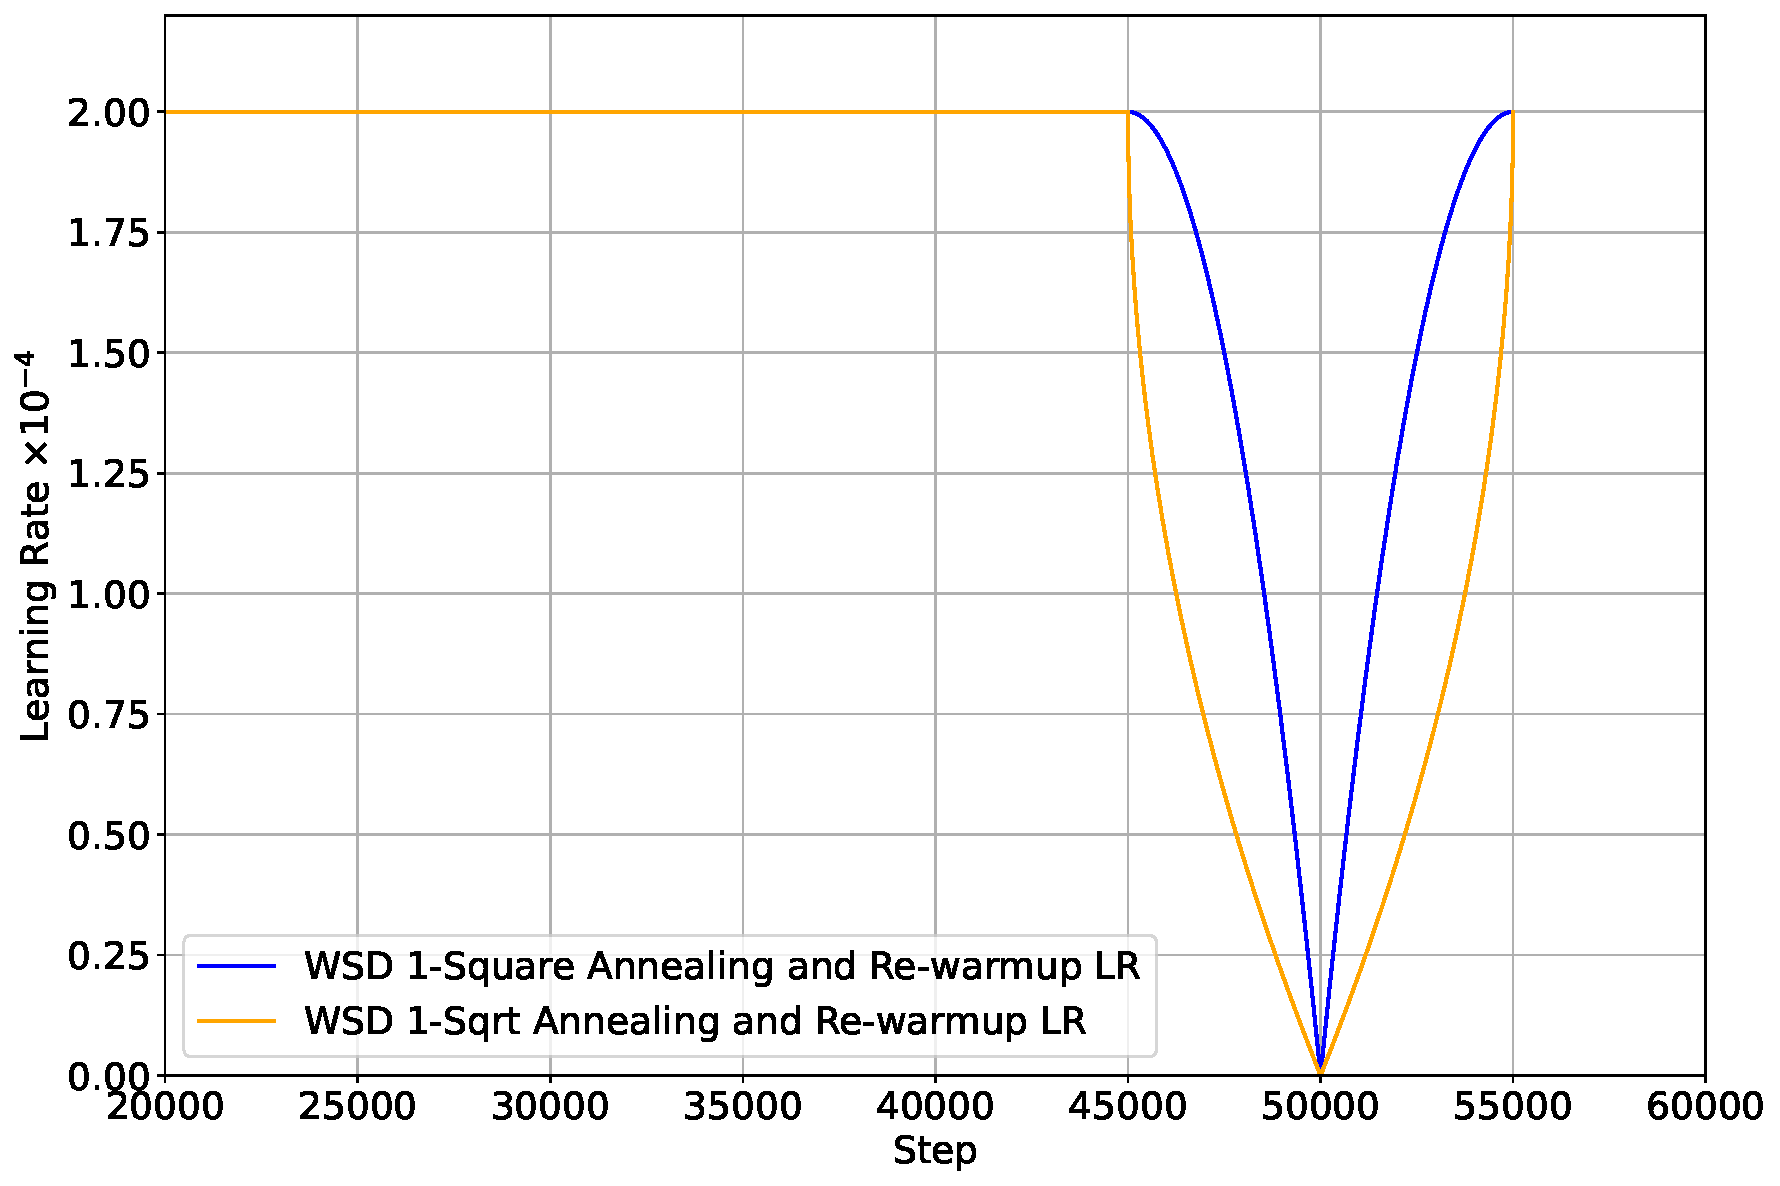
\includegraphics[width=\textwidth]{images/pdfs_0.999/wsdw_lr.pdf}
        \caption{Learning rate curves. }
    \end{subfigure}
    \hfill
    \begin{subfigure}[b]{0.32\textwidth}
        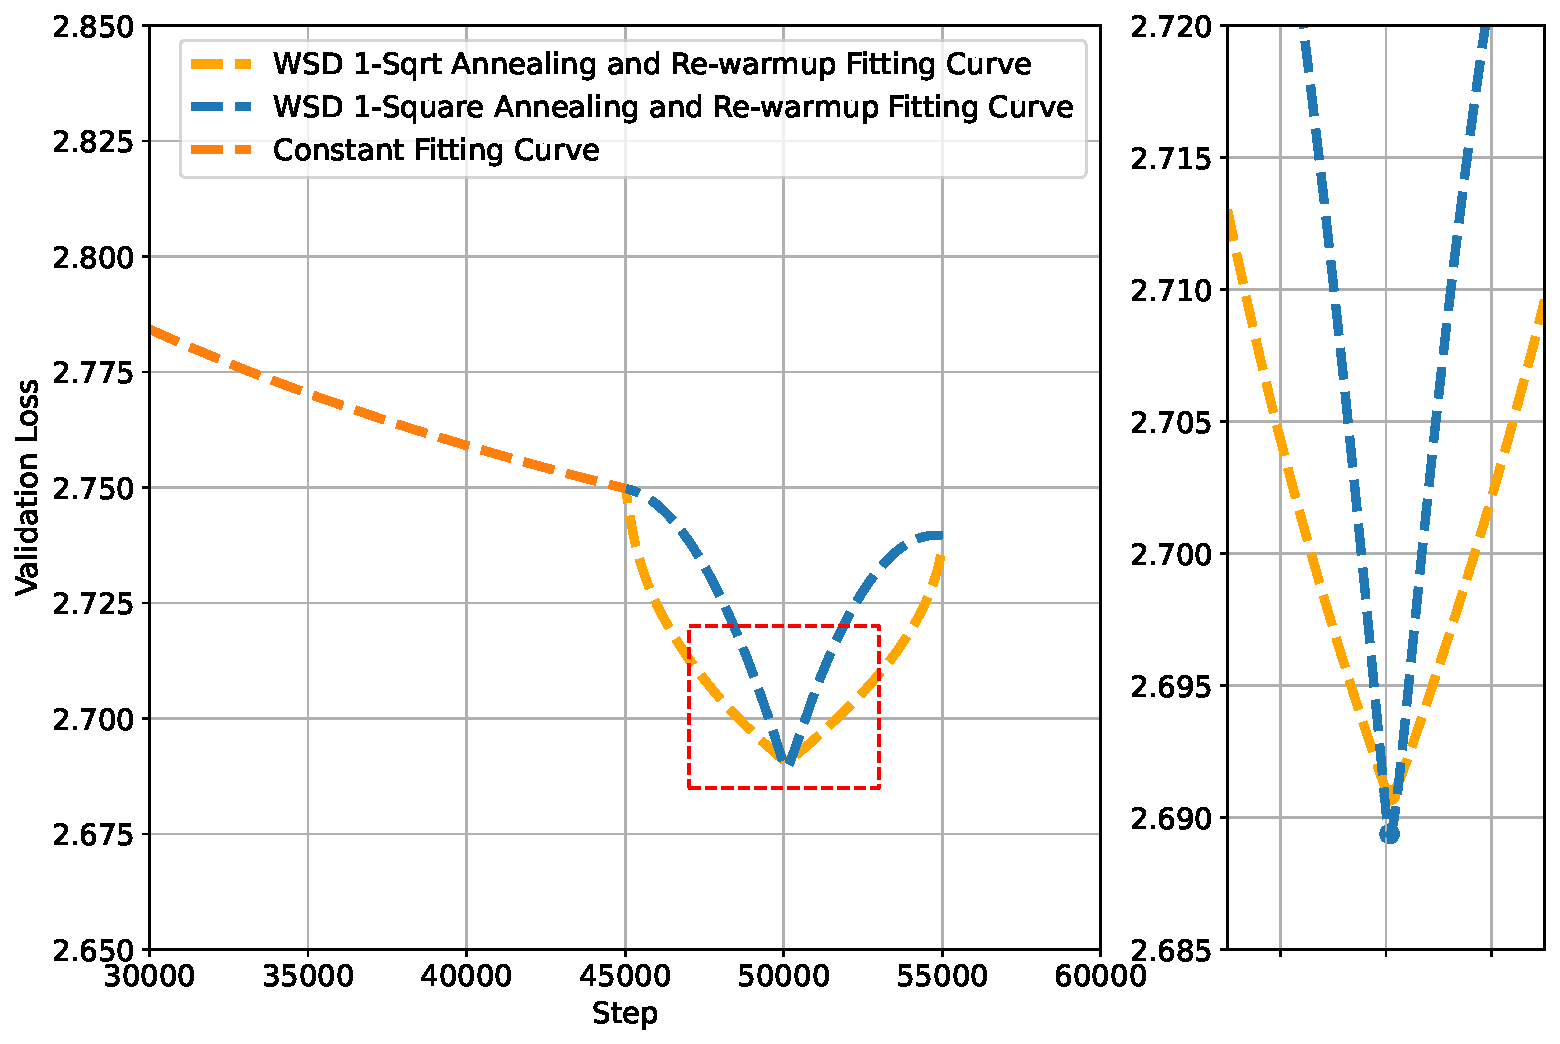
\includegraphics[width=\textwidth]{images/pdfs_0.999/predict_zoomout_lamda_99.pdf}
        \caption{The loss curve of $\lambda = 0.99$.}
        \label{fig:lambda99}
    \end{subfigure}
    \hfill
    \begin{subfigure}[b]{0.32\textwidth}
        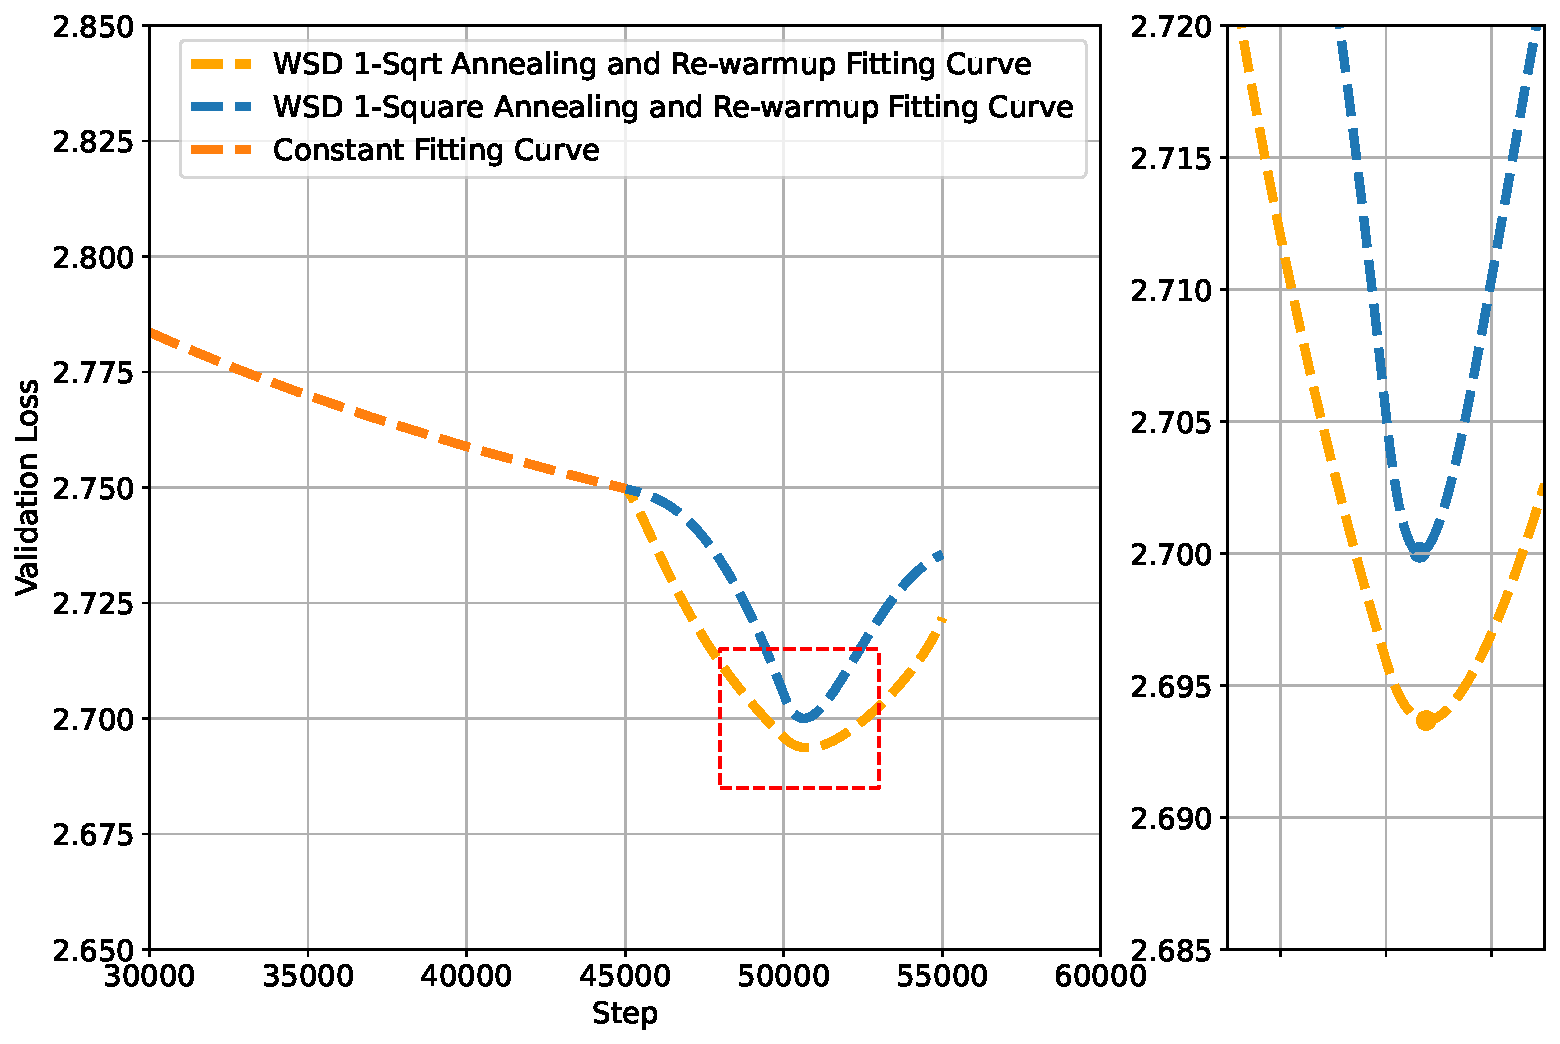
\includegraphics[width=\textwidth]{images/pdfs_0.999/predict_zoomout_lamda_999.pdf}
        \caption{The loss curve of $\lambda = 0.999$. }
        \label{fig:lambda999}
    \end{subfigure}
    \caption{The comparison of fitting effect of different decay factor $\lambda$.}
    
\label{fig:lambda}
\end{figure}

\begin{figure}[tbp]
    \centering
    \begin{subfigure}[b]{0.6\textwidth}
        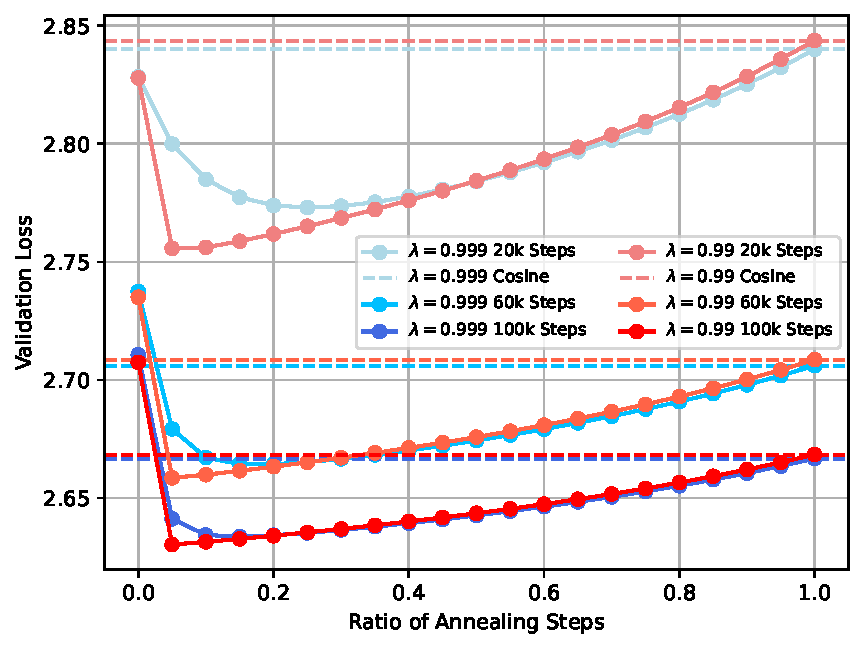
\includegraphics[width=\textwidth]{images/wsd_ratio_lamda.pdf}
    \end{subfigure}
    \caption{The predicted loss in different annealing ratios of WSD LRS for $\lambda=0.99$ and $\lambda=0.999$.}
\label{fig:wsd_lambda}
\end{figure}

The decay factor $\lambda$ in our equation indicates the information retaining degree in LR annealing. We set $\lambda$ as $0.999$ in our all experiments. We explore the difference from another decay factor $\lambda=0.99$. We fit and get different equations for different $\lambda$. We compare them (1) on the predicted loss curves for 1-square and 1-sqrt annealing methods, and (2) on the predicted loss curves in different annealing ratios of WSD LRS (cosine annealing).

The results, illustrated in Fig.~\ref{fig:lambda} and~\ref{fig:wsd_lambda}, reveal several key insights into the impact of decay factor:

\paragraph{Delay Steps.} A larger decay factor results in longer delay steps. Comparing 
Fig.~\ref{fig:lambda99} and Fig.~\ref{fig:lambda999}, $\lambda=0.999$ introduces a more obvious delay phenomenon, which is consistent across both the 1-square and 1-sqrt annealing methods.
The root reason is simple: larger $\lambda$ can retain more LR historical momentum, causing longer delay steps after LR finish annealing.

\paragraph{Optimal Annealing Ratio.} a larger decay factor tends to favor a higher annealing ratio. As shown in Fig.~\ref{fig:wsd_lambda},  
The optimal annealing ratio of $\lambda=0.999$
is larger than that of $\lambda=0.99$. Meanwhile, due to the similar reason, $\lambda=0.999$ favors 1-sqrt annealing method while $\lambda=0.99$ favors 1-square annealing method, as shown in Fig.~\ref{fig:lambda}.

\paragraph{Balance Point between $S_1$ and $S_2$.} More essentially, the selection of $\lambda$ decides the balance point of $S_1$ and $S_2$.
For example,
$\lambda=0.999$ means that LR annealing only retain the information of previous approximately $\frac{1}{1-\lambda}=1000$ steps, which can be seen as the window size of LR annealing momentum. The window size could be very close to the optimal annealing steps if LR changes smoothly over steps. After reaching window size, $S_2$ increases very slowly, with the cost of large decrease of $S_1$.

The analyses above highlights the importance of selecting a decay factor that aligns closely with empirical data to ensure the accuracy of predictions. 
We recommend that the future developers try different $\lambda$ for their own setups~\footnote{Actually, $\lambda$ can be fitted as a parameter, instead of a hyper-parameter requiring manual tuning. We regard $\lambda$ as a hyper-parameter because $\lambda=0.999$ performs well in our all experiments. Besides, fitting with $\lambda$ could bring in additional time complexity due to the recomputation of $S_2$.}.



\subsection{Possible Root Reasons of Delay Phenomenon in Learning Rate Annealing}
\label{sec:discsussion-delay}


In Sec.~\ref{sec:theorem}, we discover the delay phenomenon, which proves that LR annealing has momentum. 
We discuss possible root reasons of the phenomenon in this section.

\paragraph{Adam Optimizer? No.} We notice that Adam optimizer~\citep{adam-optim} also has the first-order momentum decay factor $\beta_1$ and the second-order momentum decay factor $\beta_2$, which presents the possible connection to the the delay phenomenon.

We keep $\beta_1=0.9$, and conduct delay experiments
on different $\beta_2 \in \{0.95, 0.99, 0.999\}$ (default: $0.95$) of AdamW optimizer~\citep{loshchilov2017decoupled} to observe whether larger $\beta_2$ causes a more longer delay steps.
The learning rate and ground-true loss curve are shown in Fig.~\ref{fig:adam_diff}. It suggests that the ground-truth loss curves of different $\beta_2$ almost coincide with each other, and their delay steps are also the same. Therefore, we believe that Adam optimizer has little to do with the delay phenomenon, despite its momentum form seeming very related to our experiments. Speaking of which, we even once tried to mimic the form of Adam Optimizer to describe LR annealing momentum, attempting to discover a connection between them, but the fitting results were a mess.

\begin{figure}[tbp]
    \centering
    \begin{subfigure}[b]{0.48\textwidth}
        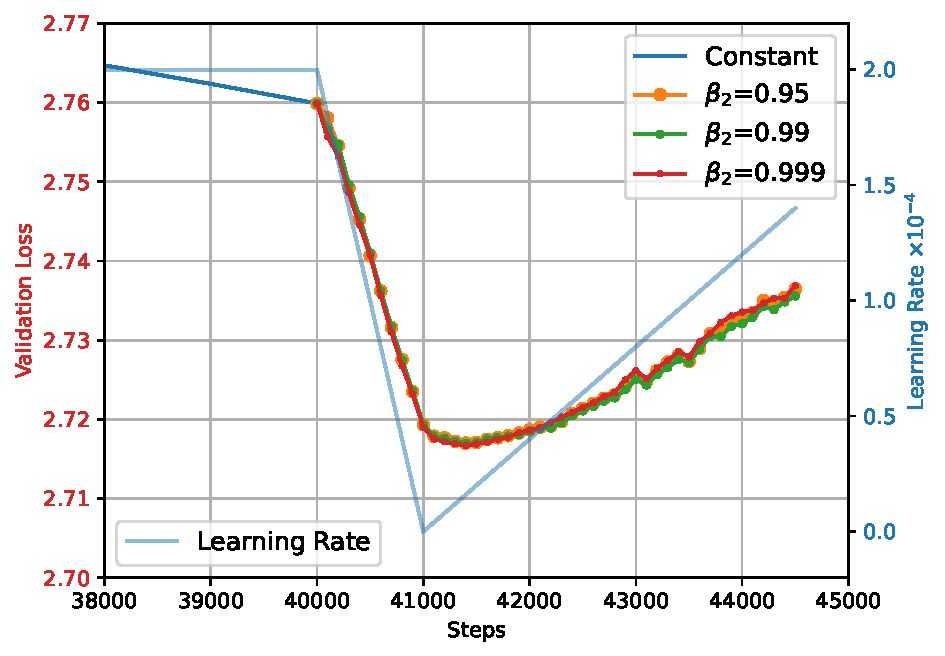
\includegraphics[width=\textwidth]{images/adma_8.pdf}
        \caption{The comparison of true loss curve with setting different $\beta_2$ of Adam optimizer.}
        \label{fig:adam_diff}
    \end{subfigure}
    \hfill
    \begin{subfigure}[b]{0.48\textwidth}
        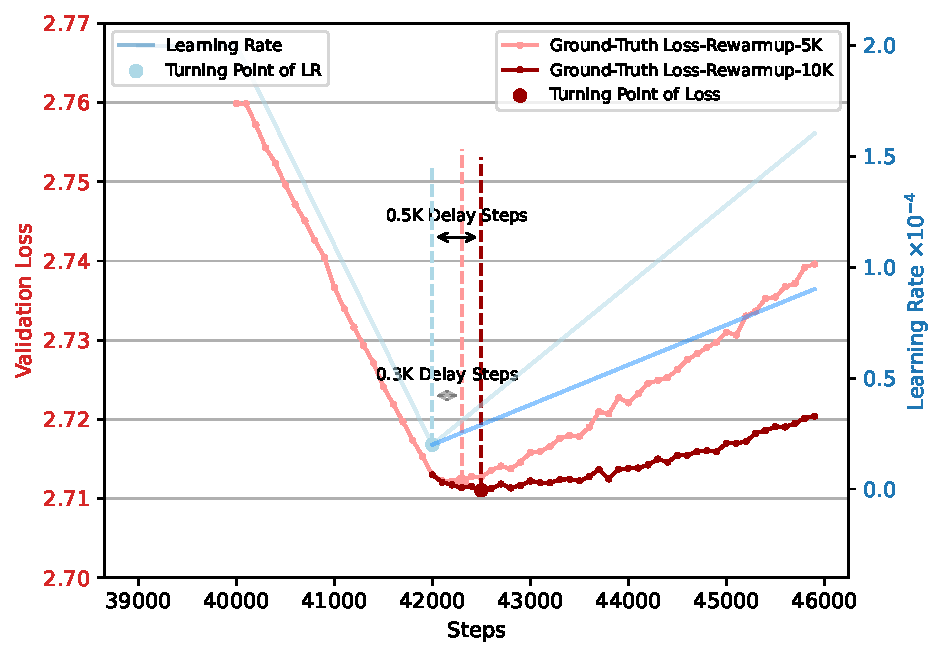
\includegraphics[width=\textwidth]{images/decrease_increase.pdf}
        \caption{The comparison of delay steps of  different re-warmup steps (and thus different $S_1$).}
        \label{fig:delay-exp-apx}
    \end{subfigure}
    \caption{The possible root reason analysis (left: Adam optimizer, right: $S_1$) of delay phenomenon.}
\label{fig:root-reason}
\end{figure}


% \begin{figure}[tbp]
%     \centering
%     \begin{subfigure}[b]{0.7\textwidth}
%         \includegraphics[width=\textwidth]{images/adma_diff.pdf}
%     \end{subfigure}
%     \caption{The comparison of true loss curve with setting different $\beta_2$ of Adam optimizer.}
% \label{fig:adam_diff}
% \end{figure}

% \begin{figure}[tbp]
%     \centering
%     \begin{subfigure}[b]{0.7\textwidth}
%         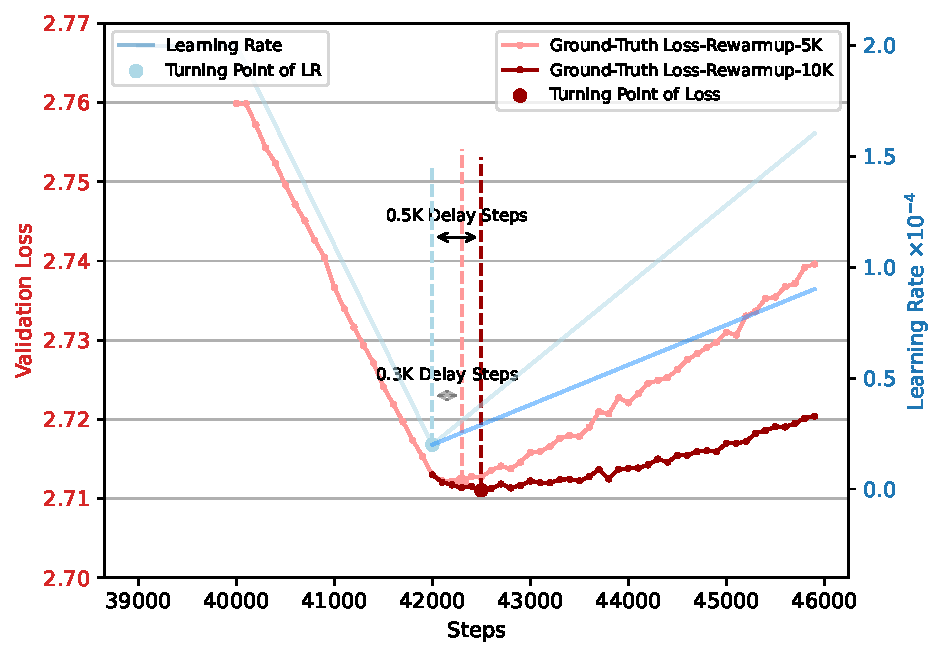
\includegraphics[width=\textwidth]{images/decrease_increase.pdf}
%     \end{subfigure}
%     \caption{The comparison of delay steps of  different re-warmup steps.}
% \label{fig:delay-exp-apx}
% \end{figure}

\paragraph{Forward Area $S_1$? Not Really.} No matter how LR changes, $S_1$ is always increasing over steps, resulting in consistently reducing the validation loss brought from $S_1$. Therefore, the forward area, $S_1$ would lengthen delay steps in LR annealing then re-warmup, but would shorten delay steps in LR re-warmup then annealing. The delay phenomenon is indeed related to $S_1$.

But still, $S_1$ is not all the reasons of delay phenomenon. We prove this by Fig.~\ref{fig:delay-rewarmup-then-anneal}, which suggests that even though in LR re-warmup then annealing, the delay phenomenon, while not that pronounced, still exists. Moreover, we conduct delay experiments by adjusting the slope of LR after tuning point of LR. As shown in Fig.~\ref{fig:delay-exp-apx}, We find that more smooth slope of LR re-warmup, with smaller $S_1$, but still causes longer delay steps. Therefore, we conclude that $S_1$ indeed influences the specific delay length, but is not the root reason.

\paragraph{Other Possible Reasons?} The delay phenomenon could be intuitive in some cases. For example, suppose that learning rate decreases directly from 2e-4 to 2e-5 in one step, and then maintains 2e-5. In this case, although the loss would decrease to a lower value but the parameter changes in one step is too small in neural networks. Given a sudden low LR, neural networks still require some steps to gradually optimize to a local minimum, incurring delay phenomenon. 
But still, analysis above still ends with a rough description, and we have not figured out the root reasons and look forward to completing this part in future work.


\subsection{Other Possible Scaling Law Formats with LR annealing}
\label{apx:discsussion-format}
\paragraph{Adding a LR-weighted Coefficient to $S_2$?}
Imagine that when LR anneals to nearly $0$, the neural network's parameters almost do not change and the validation loss should not change, either.
However, as defined in our equation, Eq.~\ref{eq:scaling}, $S_2$ still has historical momentum even if LR is nearly $0$, making the loss continue to decrease and misalign with observed training dynamics.

To cover this corner case, we try a revision to our equation and add a LR-weighted coefficient to $S_2$. Specifically, we adjust $S_2$ to more approach $0$ when $\eta$ is close to $0$, counteracting the original formulation's tendency to overestimate loss reduction when $\eta\approx0$. 

% This modification aims to more accurately reflect the diminishing effectiveness of learning rate changes as they near zero, aligning the predicted loss curve more closely with observed training behaviors.

The revised equation for the annealing area \(S_2\) in our scaling law function is as follows:
\begin{equation}
\label{eq:scaling_withlr}
\begin{aligned}
m_i &= \lambda\cdot m_{i-1} + (\eta_{i-1} - \eta_{i}) \\
&= \sum\limits_{k=1}^{i}(\eta_{k-1} - \eta_{k})\cdot \lambda^{i-k}, \\
S_2 &= \sum\limits_{i=1}^{s} m_i \color{red}\cdot \eta_{i}^{\epsilon},
\end{aligned}
\end{equation}
where the red part is the added LR-weighted coefficient and $\epsilon$ is a undetermined positive constant. $\epsilon$ could be very small in practice.

We have tried the revised function to fit data. We find that the fitting results are quite similar and $\epsilon$ is very close to 0, showing little use in practical effect. Hence, we adopt the original format in our experiments. However, we still recommend future developers to try this format if possible.

\paragraph{$L \propto S_2^{\zeta}$ rather than {$L \propto S_2$}?}



\begin{figure}[tbp]
    \centering
    \begin{subfigure}[b]{0.32\textwidth}
        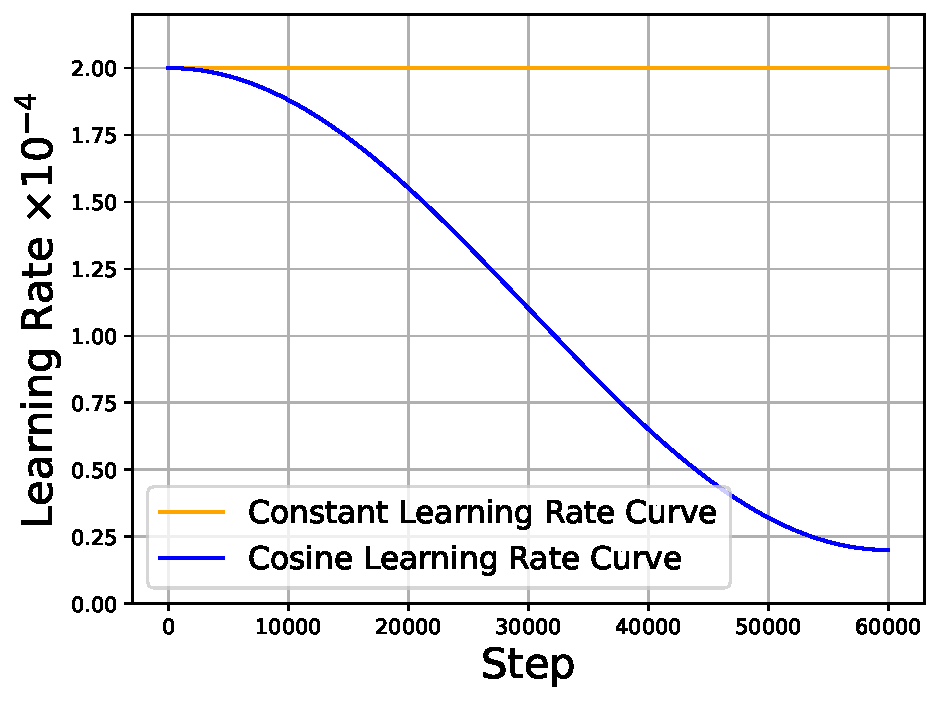
\includegraphics[width=\textwidth]{images/plot_newxy/eta_lr_1.pdf}
        \caption{LR of cosine and constant. }
    \end{subfigure}
    \hfill
    \begin{subfigure}[b]{0.32\textwidth}
        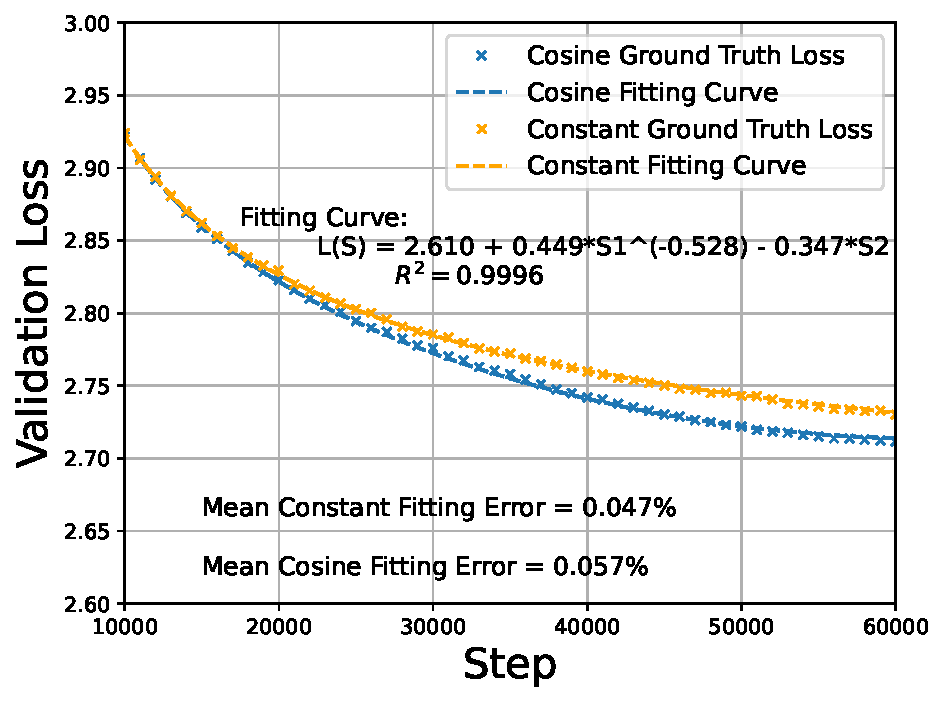
\includegraphics[width=\textwidth]{images/plot_newxy/predict_zoomout_noeta_2.pdf}
        \caption{The fitting curve of $L \propto S_2$}
    \end{subfigure}
    \hfill
    \begin{subfigure}[b]{0.32\textwidth}
        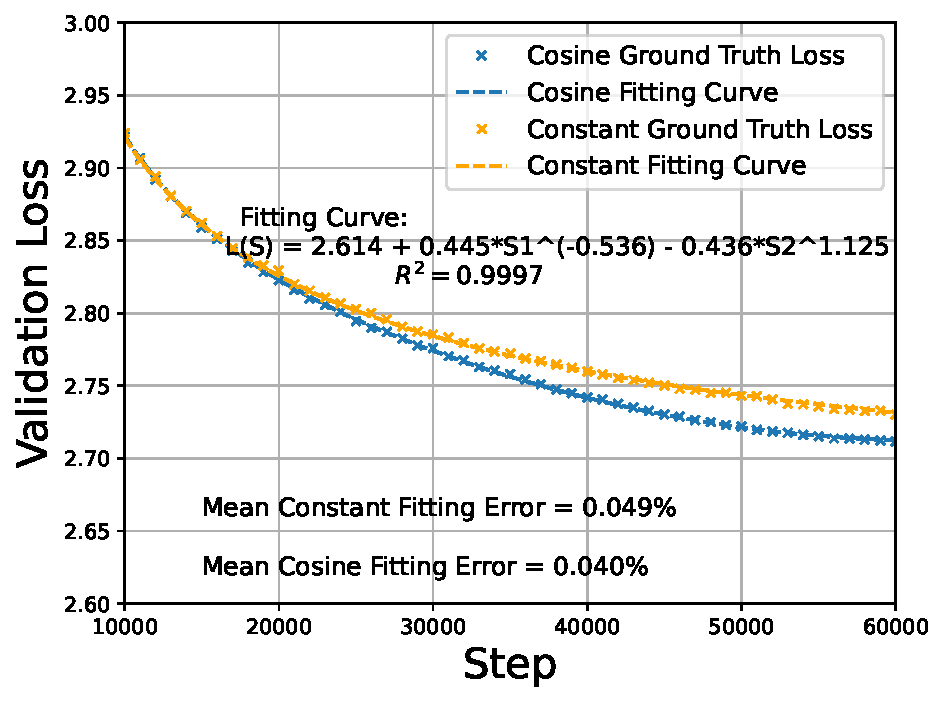
\includegraphics[width=\textwidth]{images/plot_newxy/predict_zoomout_eta_2.pdf}
        \caption{The fitting curve of $L \propto S_2^{\zeta}$. }
        \label{fig:have-zeta}
    \end{subfigure}
    \caption{The comparison of fitting effect between $L \propto S_2^{\zeta}$ with $L \propto S_2$.}
    
\label{fig:zeta}
\end{figure}

Actually, all we know is that $L$ and $S_2$ have a positive correlation. Thus $L\propto S_2^\zeta$ rather than $L \propto S_2$ might be a more reasonable assumption. 
That is, our equation would be changed to 
$L(s) = L_0 + A\cdot S_1^{-\alpha} - C\cdot S_{2}^{{\color{red} \zeta}} $.
Theoretically, the introduction of \(\zeta\) as an additional fitting parameter is expected to provide a more nuanced control over how changes in the learning rate annealing affect validation loss, potentially leading to improve the accuracy of our equation. 

However, the empirical results, as depicted in Fig.~\ref{fig:zeta}, demonstrate that the fitting improvement with the inclusion of \(\zeta\) is quite marginal when compared to the version without this parameter. This slight enhancement does not justify the additional complexity introduced by managing negative values of \(S_2\). Furthermore, the empirical observation that \(\zeta\) tends to converge close to $1$ (e.g. $1.125$ in Fig.~\ref{fig:have-zeta}) reinforces the notion that the original formulation of the function, without the power term \(\zeta\), is adequately robust. This finding suggests that the direct influence of the learning rate annealing area, as initially modeled, sufficiently captures the essential dynamics without the need for this additional complexity. Another additional complexity lies in that $S_2^{\zeta}$ becomes incalculable when $S_2<0$ in LR re-warmup.
